\documentclass[]{article}
\usepackage[round]{natbib}

\usepackage{fullpage}
\usepackage{listings}
\usepackage{url}
\usepackage{authblk}
\usepackage{graphicx}
\usepackage{color}
\usepackage{booktabs}

\lstset{language=Python}

% local definitions
\newcommand{\comment}[1]{{\textcolor{red}{Comment: #1}}}

% cross-reference with supplement
\usepackage{xr}
\externaldocument{supplement}

\begin{document}

\title{An article template}
\author[1,*]{The Author}
\affil[1]{Planet Earth}
\affil[*]{email@address.edu}
\maketitle

\begin{abstract}
A very simple template for an article class document.
\end{abstract}

\section{Interpretation of results}

\begin{enumerate}
    \item Human generation time differences between populations are claimed
        to extend to more than 250,000 years. Extending the analysis beyond
        10,000 generations shows that generation times do not converge
        until ``78,000'' generations ago (more than 2 million years).
        This is implausible.
    \item Eurasian--West African divergence has been estimated to be around
        \citep[e.g.,][]{pagani2015tracing}
    \item Even papers that have inferred deep divergences of human populations
        in Africa would place the West Africa--Eurasian divergence around
        100--150ka \citep[e.g.,][]{schlebusch2017southern}.
    \item It's worth noting that multiple studies have found evidence for
        deep population structure in the history of Bantu-speaking groups.
        However, it's unclear if such structure could account for such
        long-lasting differences in generation times, or if that structure
        is mis-inferred (as we argue in \citet{ragsdale2022weakly}).
\end{enumerate}

\section{The mutation spectrum over time}

Issues:
\begin{enumerate}
    \item GEVA-Atlas variant ages result in mutation spectra that change
        rapidly beyond 10,000 generates (which is likely why the weren't
        shown?)
    \item Allele age estimates between three state-of-the-art methods
        [\texttt{GEVA} \citep{albers2020dating}, Relate
        \citep{speidel2019method}, and \texttt{tsdate}
        \citep{wohns2022unified}] are only moderately correlated
        (for example, see Figure S20 in the Supplement of
        \citet{wohns2022unified}).
    \item Allele ages provided by each method results in distinct and
        unalike mutation spectrum histories
        (Figures~\ref{fig:geva-spectra}--\ref{fig:relate-spectra}).
    \item In turn, these divergent histories provide estimates of
        generation time profiles that differ completely.
\end{enumerate}

\section{De novo mutations from trio data}

\begin{enumerate}
    \item \emph{De novo} mutations from the Icelandic trio study have
        a different mutation profile than the most recent age bins
        (across all three of the variant dating methods).
    \item In the most recent age bins (0 to 50 or 80 generations ago),
        the three methods estimate very similar spectra of young standing
        variation. They are closer to each other than any of them are
        to the spectrum from \citet{jonsson2017parental}.
    \item \citet{wang2023human} acknowledge this:
        \begin{quote}
            We found that the mutation spectrum from the large pedigree study
            (14) consistently differed from the variant spectrum inferred from
            the 1000 Genomes Project data, possibly because we removed
            singletons from the polymorphism dataset to reduce errors.''
        \end{quote}
    \item However, they did not test (or at least did not show a test of)
        this hypothesis that the removal of singletons drives this signal.
        I don't think it does, but want to dive into it a bit more
        thoroughly.
        \comment{Update: GEVA does not provide ages for singletons. Relate
            and tsdate do, however, so we can test this hypothesis there.}
    \item Table~\ref{tab:recent-spectra} shows mutation spectrum from the
        most recent bin in each dataset.
    \item I also don't think the approach they took is satisfying:
        \begin{quote}
            Therefore, to obtain absolute generation times for historical
            periods, we centered the observed spectra on the most recent bin,
            subtracting its difference with the average mutation spectrum
            estimated in (14) from each historical spectrum.  This has the
            effect of assuming that parental ages in the pedigreed mutation
            dataset reflect generation times in the most recent historical bin.
        \end{quote}
        And I don't know what biases this introduces. It does have the effect
        of forcing recent bins to have roughly the same inferred average
        generation times for mothers and fathers as the iceland trio data
        ($28.2$ and $32$, resp.). It's therefore not a \emph{result} that
        recent time periods match other estimates. It's a built-in assumption
        of their model
\end{enumerate}

\section{Bigger picture issues and commentary}

\begin{enumerate}
    \item Allele age estimates are noisy, and probably shouldn't be used
        for such detailed inferences. You'll end up fitting the noise and
        bias of each method.
    \item DNM estimates from trios have their own sets of problems. Do we
        know where the discrepancy between trio-estimated DNM spectrum and
        observations from pop-gen data come from? Probably needs to be
        sorted out.
\end{enumerate}

\break

\section{Figures}

\begin{figure}[ht!]
    \centering
    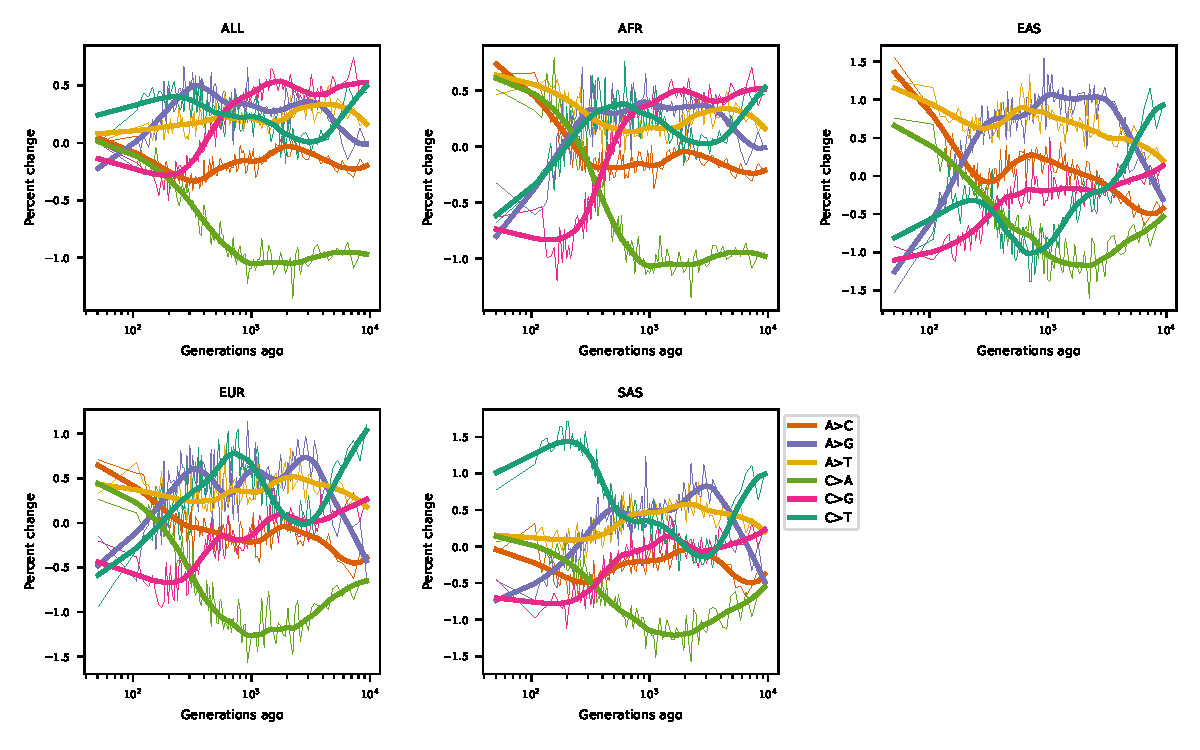
\includegraphics[width=0.8\textwidth]{../plots/spectrum_history.geva.max_age.10000.pdf}
    \caption{
        \textbf{\texttt{GEVA}-inferred mutation spectrum history.}
    }
    \label{fig:geva-spectra}
\end{figure}


\begin{figure}[ht!]
    \centering
    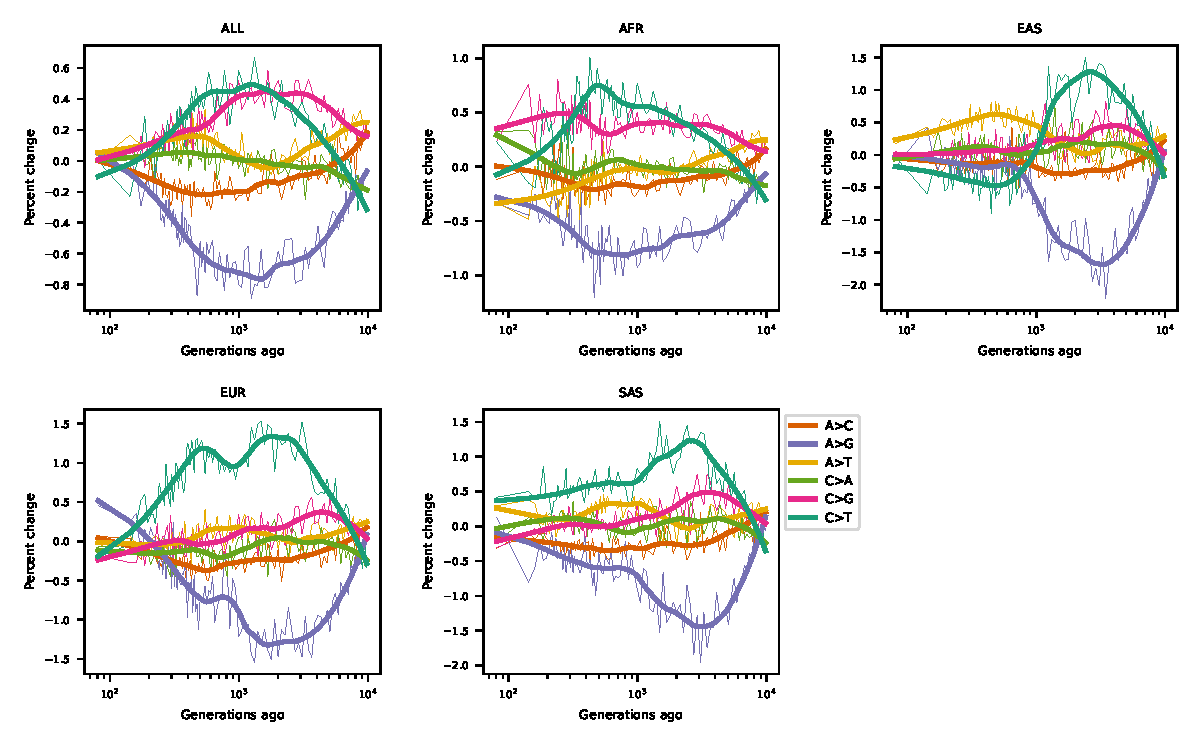
\includegraphics[width=0.8\textwidth]{../plots/spectrum_history.relate.max_age.10000.pdf}
    \caption{
        \textbf{\texttt{Relate}-inferred mutation spectrum history.}
    }
    \label{fig:relate-spectra}
\end{figure}


\begin{figure}[ht!]
    \centering
    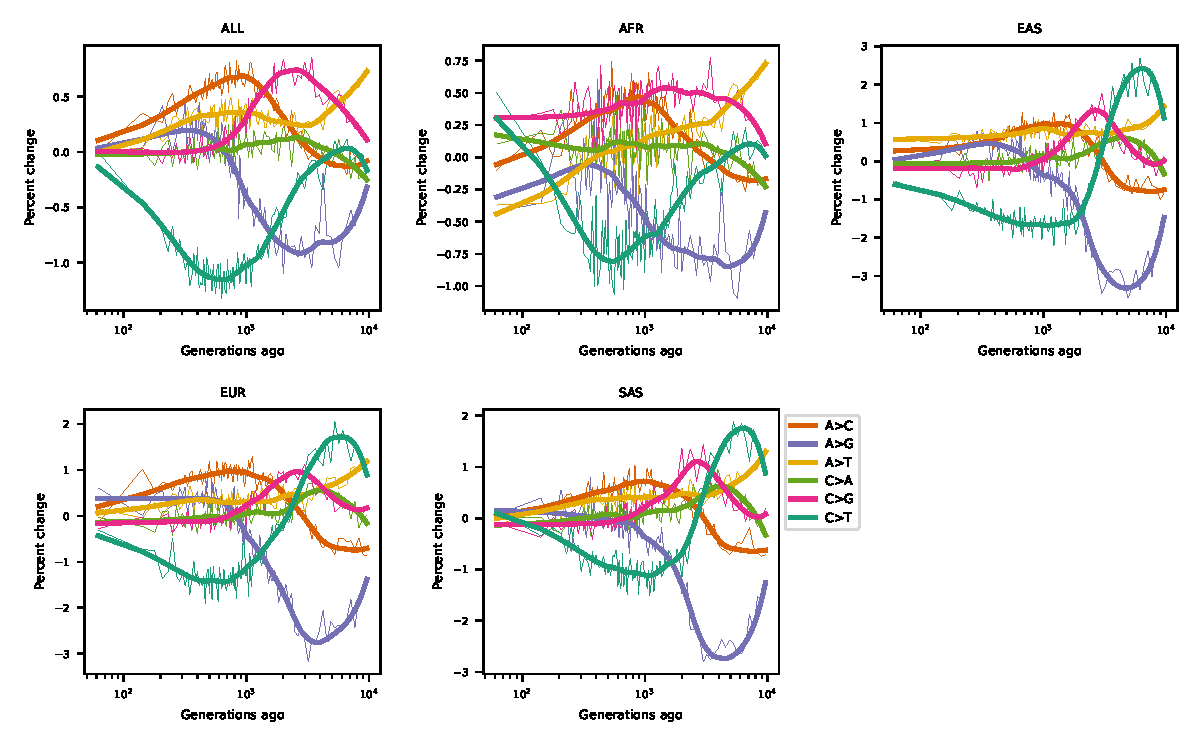
\includegraphics[width=0.8\textwidth]{../plots/spectrum_history.tsdate.max_age.10000.pdf}
    \caption{
        \textbf{\texttt{tsdate}-inferred mutation spectrum history.}
    }
    \label{fig:tsdate-spectra}
\end{figure}


\begin{figure}[ht!]
    \centering
    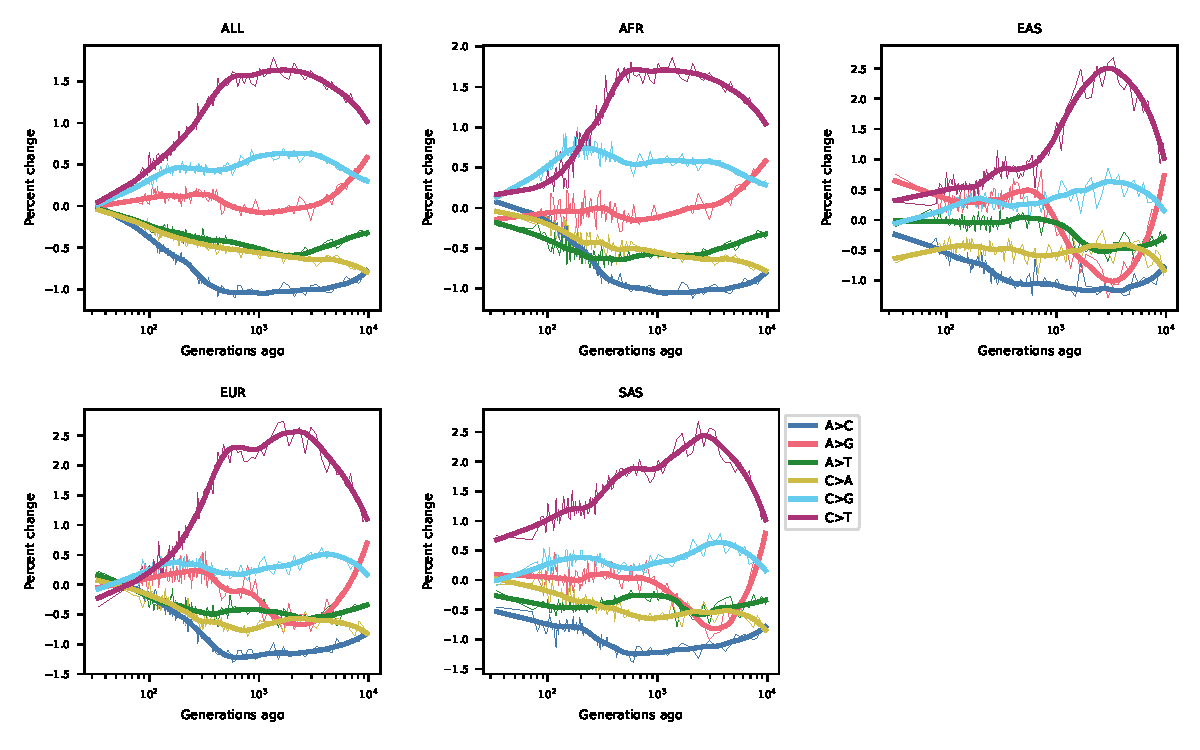
\includegraphics[width=0.8\textwidth]{../plots/spectrum_history.relate.max_age.10000.singletons.pdf}
    \caption{
        \textbf{\texttt{Relate}-inferred mutation spectrum history, including singletons.}
    }
    \label{fig:relate-spectra}
\end{figure}


\begin{figure}[ht!]
    \centering
    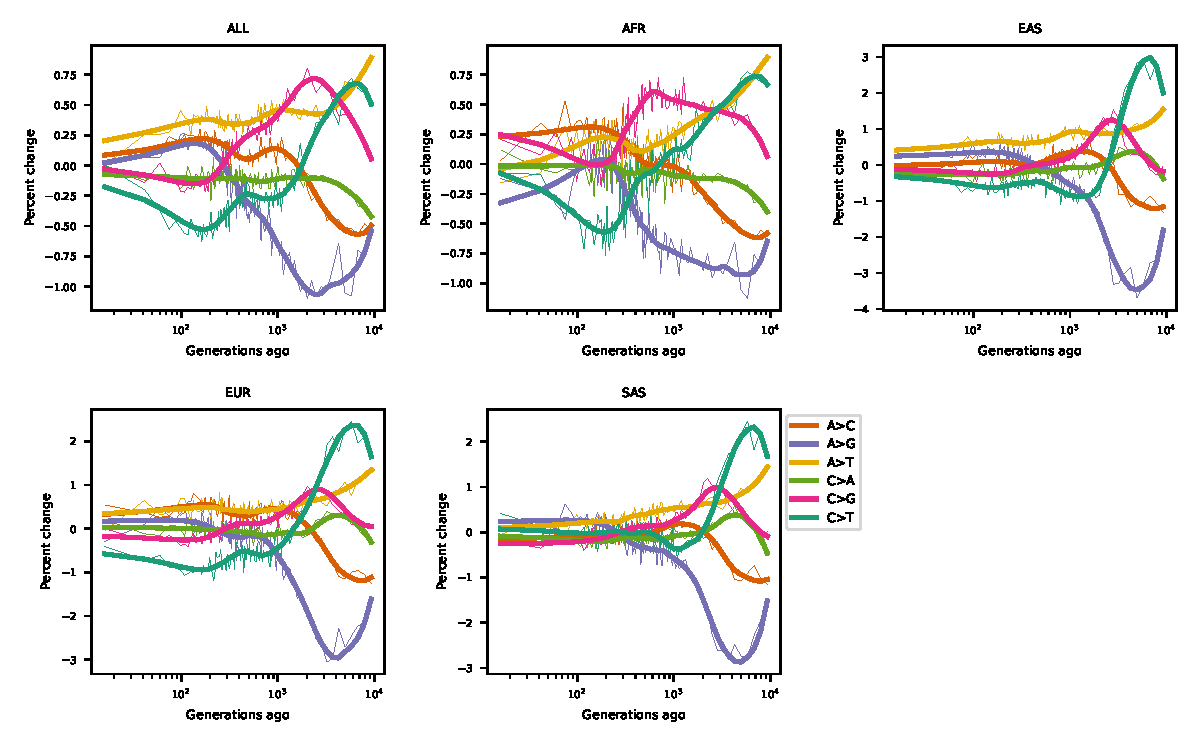
\includegraphics[width=0.8\textwidth]{../plots/spectrum_history.tsdate.max_age.10000.singletons.pdf}
    \caption{
        \textbf{\texttt{tsdate}-inferred mutation spectrum history, including singletons.}
    }
    \label{fig:tsdate-spectra}
\end{figure}


\begin{figure}[ht!]
    \centering
    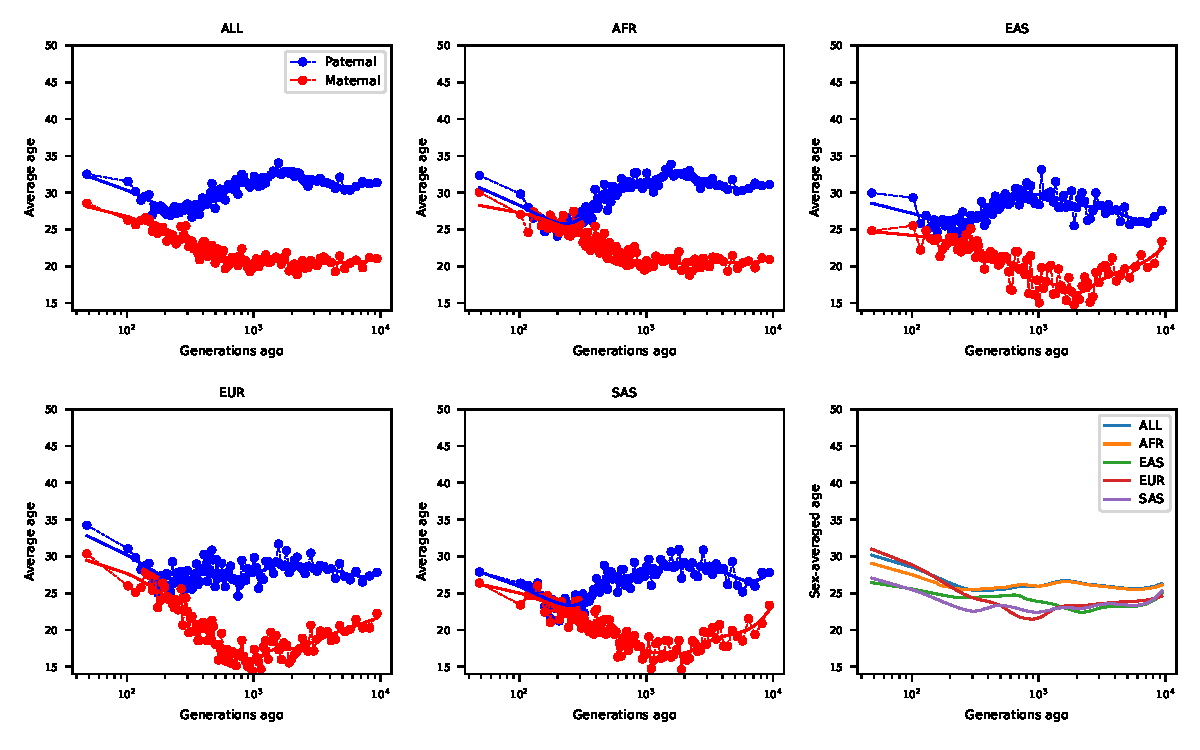
\includegraphics[width=0.8\textwidth]{../plots/inferred_generation_times.geva.pdf}
    \caption{
        \textbf{\texttt{GEVA}-inferred generation time histories.}
    }
    \label{fig:geva-gen-times}
\end{figure}


\begin{figure}[ht!]
    \centering
    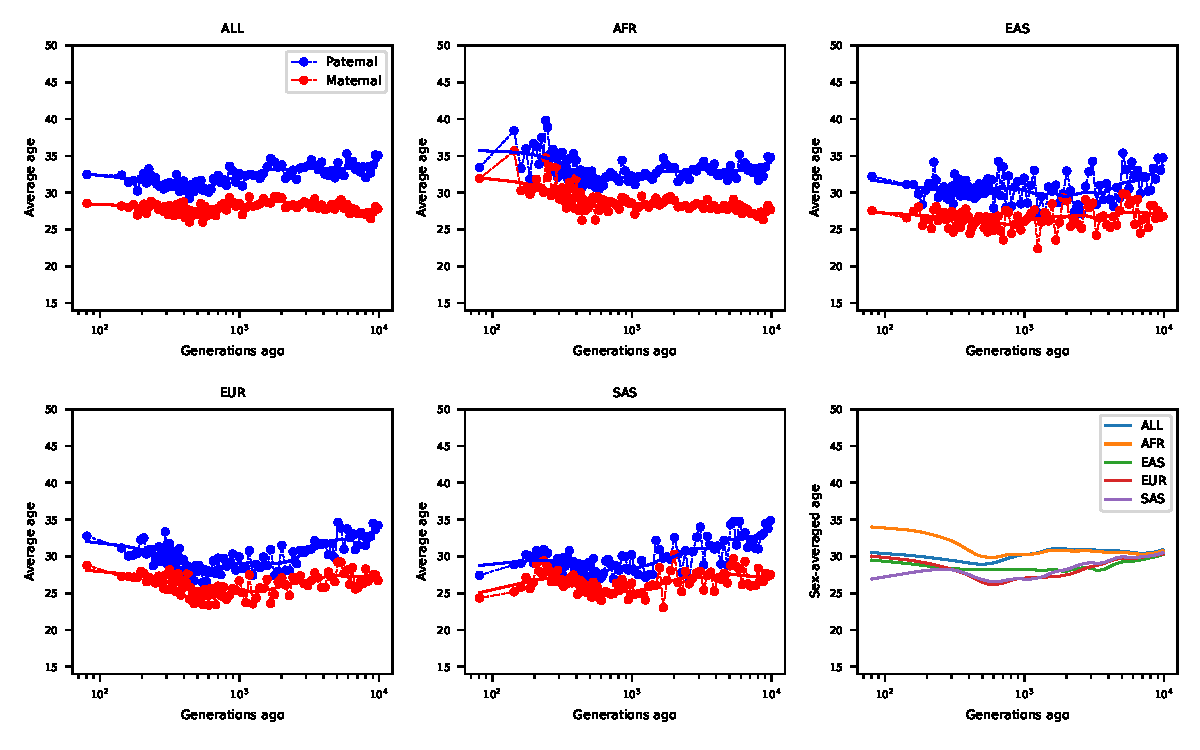
\includegraphics[width=0.8\textwidth]{../plots/inferred_generation_times.relate.pdf}
    \caption{
        \textbf{\texttt{Relate}-inferred generation time histories.}
    }
    \label{fig:relate-gen-times}
\end{figure}


\begin{figure}[ht!]
    \centering
    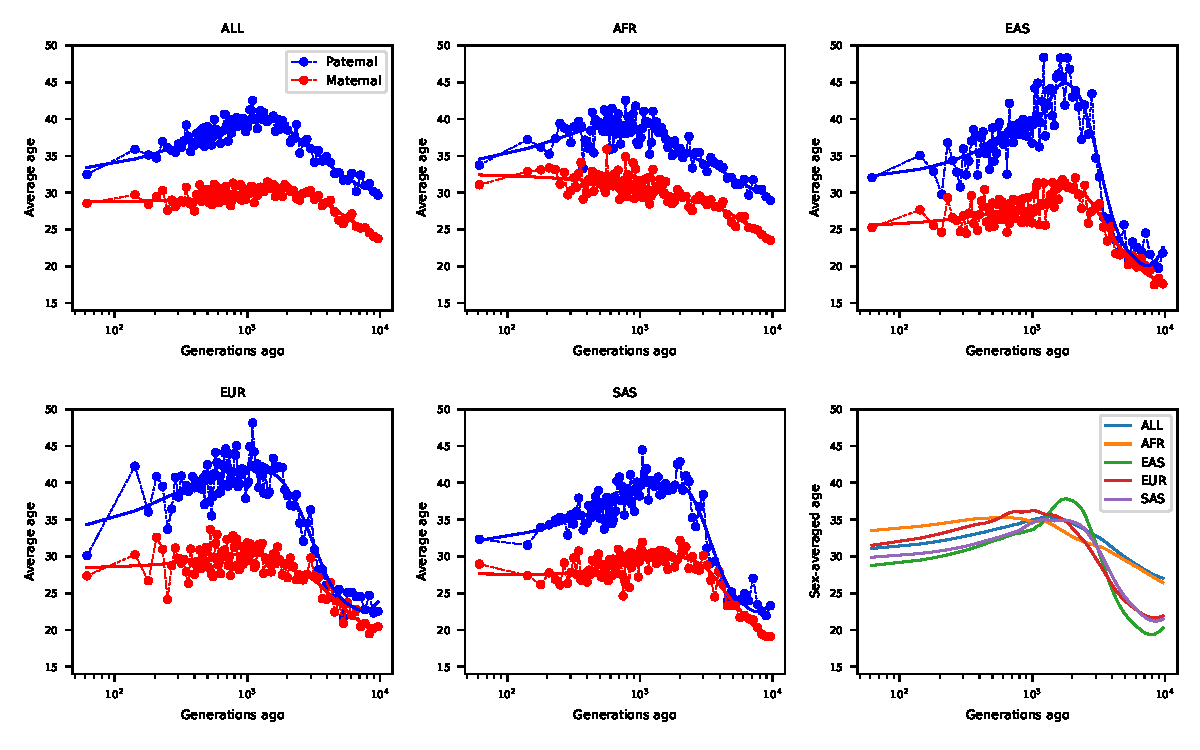
\includegraphics[width=0.8\textwidth]{../plots/inferred_generation_times.tsdate.pdf}
    \caption{
        \textbf{\texttt{tsdate}-inferred generation time histories.}
    }
    \label{fig:tsdate-gen-times}
\end{figure}


\begin{figure}[ht!]
    \centering
    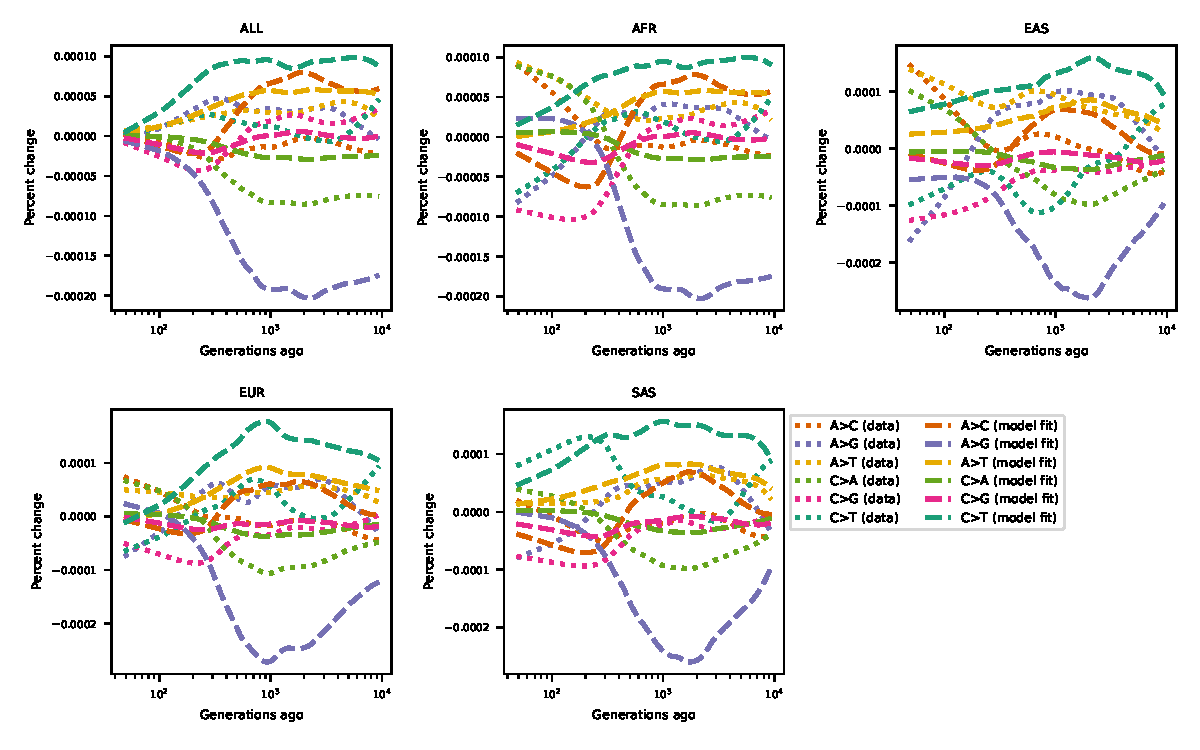
\includegraphics[width=0.8\textwidth]{../plots/goodness-of-fit.geva.pdf}
    \caption{
        \textbf{Prediction of mutation spectrum history from
        \texttt{GEVA}-inferred generation times.}
    }
    \label{fig:geva-fit}
\end{figure}


\begin{figure}[ht!]
    \centering
    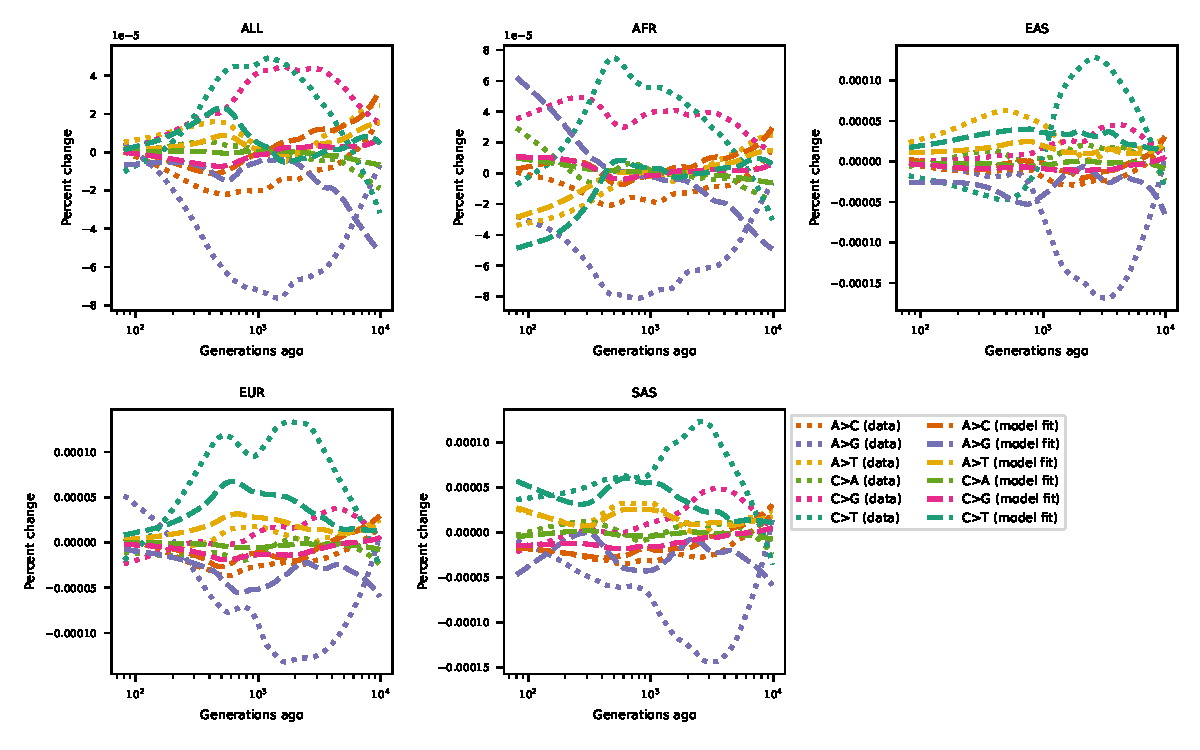
\includegraphics[width=0.8\textwidth]{../plots/goodness-of-fit.relate.pdf}
    \caption{
        \textbf{Prediction of mutation spectrum history from
        \texttt{Relate}-inferred generation times.}
    }
    \label{fig:relate-fit}
\end{figure}


\begin{figure}[ht!]
    \centering
    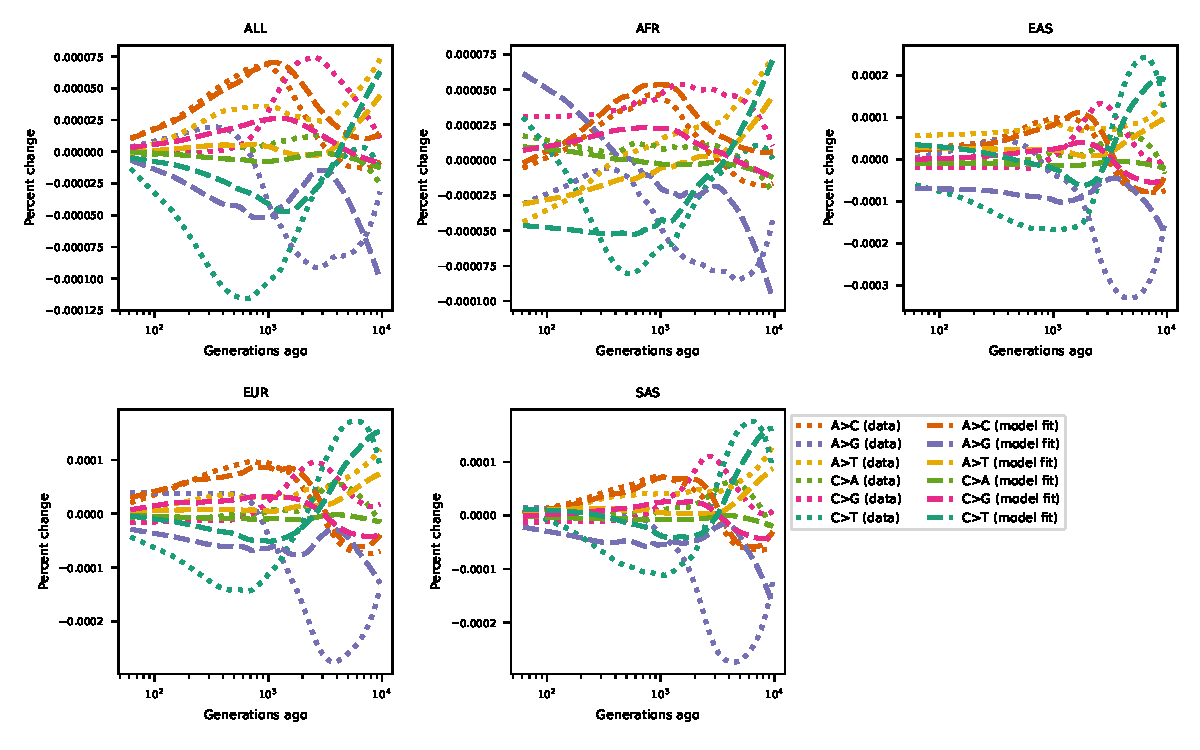
\includegraphics[width=0.8\textwidth]{../plots/goodness-of-fit.tsdate.pdf}
    \caption{
        \textbf{Prediction of mutation spectrum history from
        \texttt{tsdate}-inferred generation times.}
    }
    \label{fig:tsdate-fit}
\end{figure}


\clearpage

\section{Tables}

\begin{table}[h]
    \caption{
        \label{tab:recent-spectra}
        \textbf{Mutation profiles from the past 100 generations,
        compared to Iceland trios.}
        The most recent time bin for each method included the past $\approx150$
        generations. When singletons were included (when using data from
        \texttt{tsdate} and \texttt{Relate}), the spectra of estimated
        recent standing variation were largely similar. Note that \texttt{GEVA}
        does not report ages for singletons.
        While the three methods provide similar spectra from recent mutations,
        the spectrum from the Iceland trios differs substantially.
        The similarity in the spectrum between mutations that were phased
        in \citet{jonsson2017parental} and all mutations (phased and unphased)
        are very similar to each other.
    }
    \centering
    \begin{tabular}[t]{l|cccccc}
        \toprule
        Dataset & A$\rightarrow$C & A$\rightarrow$G & A$\rightarrow$T &
            C$\rightarrow$A & C$\rightarrow$G & C$\rightarrow$T \\
        \midrule
        \texttt{GEVA} & 0.0946 & 0.3600 & 0.0886 & 0.1201 & 0.1057 & 0.2310 \\
        \texttt{tsdate} & 0.0931 & 0.3579 & 0.0899 & 0.1146 & 0.1061 & 0.2384 \\
        \texttt{tsdate} (w/singletons) & 0.0989 & 0.3598 & 0.0908 & 0.1168 & 0.1062 & 0.2275 \\
        \texttt{Relate} & 0.0991 & 0.3610 & 0.0863 & 0.1124 & 0.1038 & 0.2374 \\
        \texttt{Relate} (w/singletons) & 0.1002 & 0.3590 & 0.0921 & 0.1164 & 0.1060 & 0.2263 \\
        \midrule
        Trios (phased) & 0.1071 & 0.4100 & 0.0881 & 0.0481 & 0.0847 & 0.2620 \\
        Trios (all mutations) & 0.1080 & 0.4086 & 0.0903 & 0.0483 & 0.0839 & 0.2610 \\
        \bottomrule
    \end{tabular}
\end{table}

\clearpage

\bibliographystyle{plainnat}
\bibliography{doc}

\end{document}
